We have selected a partially made-up distribution system, located in the region of Baixo Alentejo, to further test the implementation of both the PGD and the smart contracts. Figure \ref{fig:baixo1} displays the geographical position of the 13 \textit{concelhos} forming Baixo Alentejo along with the interconnections.

\begin{figure}[!htb]\centering
    \incfig{baixo1}
    \caption{Schematic representation of the made up distribution system in Baixo Alentejo. Own elaboration. Data of the map extracted from \cite{cimbal}.}
    \label{fig:baixo1}
\end{figure}
We assume the presence of four distributed photovoltaic (PV) power plants. According to ENTSO-E, the transmission system is connected to Ferreira do Alentejo \cite{entsoe}. This will act as the slack bus of the distribution system, while the rest of the buses are load buses (also called PQ buses). Their demand is proportional to the population, whose data is extracted from \cite{wiki1}. Table \ref{tab:Sdata} presents the powers' information.

\begin{table}[!htb]\centering
    \caption{Power data for the demand and the PV generation}
    \begin{tabular}{rlrr}
        \hline
         \textbf{Bus} & \textbf{Town} & \textbf{Peak demand (MW)} & \textbf{PV installed (MW)} \\
         \hline
         1 & Ferreira do Alentejo & 5.45 & - \\
         2 & Cuba & 3.22 & - \\
         3 & Beja & 23.66 & 30.00 \\
         4 & Aljustrel & 6.11 & - \\
         5 & Alvito & 1.65 & - \\
         6 & Vidigueira & 3.92 & - \\
         7 & Castro Verde & 4.80 & - \\
         8 & Ourique & 3.55 & - \\
         9 & Almodôvar & 4.92 & 9.81 \\
         10 & Mértola & 4.80 & 8.85 \\
         11 & Serpa & 10.31 & - \\
         12 & Moura & 10.01 & 13.44 \\
         13 & Barrancos & 1.21 & - \\
        \hline
    \end{tabular}
    \label{tab:Sdata}
\end{table}
To work with non-null reactive power demands, a power factor $\cos \phi = 0.9$ has been assumed. No current limitations are imposed to keep the problem simple enough, although the PGD is perfectly capable of handling them. On the other hand, the presence of PV power plants does not imply the exclusion of PV panels installed at the residential level. However, as they are supposed to make up a tiny percentage of the total, they can be modeled as variations in demand and not purely generation sources. 

The installed PV capacity has been chosen to surpass the local peak demand. While at current times it may be hard to imagine, if renewables have to cover a large chunk of the electricity mix, this may not be far from the truth. The second reason regarding this decision is a didactic one. If PV generation were to be too small, all of its power would be consumed by the load in the bus where they are both connected. Contrarily, if PV power takes large values, decisions have to be made to prioritize power coming from Ferreiro do Alentejo (our slack bus) or from the installed PV panels. 

This way, the complex power is mathematically speaking decomposed as
\begin{equation}
	\bm{S} (\bm{x},\bm{t},\bm{p_f}) = X(\bm{x})\otimes T(\bm{t})\otimes S_d + X(\bm{x})\otimes T(\bm{t})\otimes P_g(\bm{p_f}) \ ,
\label{eq:full_case}
\end{equation}
where $X$ represents the position dimension, $T$ stands for the time dimension, $S_d$ is the known power consumption and $P_g$ corresponds to the active power generation from renewables. Note that $P_g$ depends on $\bm{p_f} \in [0,1]$. This is an array of scalars whose job is to account for variations in the PV generation. 

The demand and the PV power generation over time have profiles like the ones depicted in Figure \ref{fig:pgpd}. They have been normalized to per-unit values. The PGD considers 3 dimensions. In this case, as shown in Equation \ref{eq:full_case}, they are space, time, and variation in renewable powers. We have assumed demand is constant, although a fourth dimension could be included to parametrize it. PV generation can take any value under the bell. While each PV generation plant could be decoupled from every other, this would imply the usage of a total of 6 dimensions. To present a simple enough and didactic problem, we have assumed all PV generation sources are scaled by the same factor. 

\begin{figure}[!htb] \centering
    \begin{subfigure}[!htb]{0.45\textwidth}
        \centering
        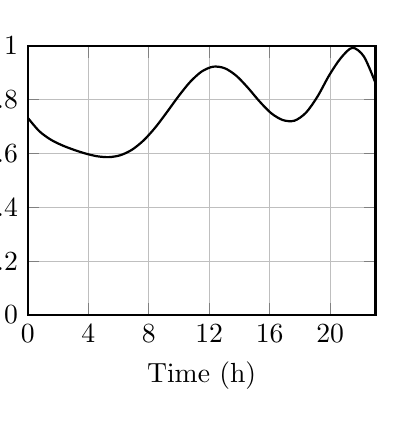
\begin{tikzpicture}[trim axis right,trim axis left,%
            declare function = {Pdemand(\y)=  0.0363*(22.394708020782733 - 1.6354720294954328*\x + 0.39434274588533585*\x*\x - 0.0035090092967717756*\x*\x*\x - 0.029337034458808153*\x*\x*\x*\x + 0.007731225380636515*\x*\x*\x*\x*\x - 0.0008557978395676469*\x*\x*\x*\x*\x*\x + 0.00004732882729208937 *\x*\x*\x*\x*\x*\x*\x - 0.00000128996363643316*\x*\x*\x*\x*\x*\x*\x*\x + 1.381540655448e-8*\x*\x*\x*\x*\x*\x*\x*\x*\x) ;}, %
            declare function = {Pdemandx(\y)=  (0.0363*(22.394708020782733 - 1.6354720294954328*\x + 0.39434274588533585*\x*\x - 0.0035090092967717756*\x*\x*\x - 0.029337034458808153*\x*\x*\x*\x + 0.007731225380636515*\x*\x*\x*\x*\x - 0.0008557978395676469*\x*\x*\x*\x*\x*\x + 0.00004732882729208937 *\x*\x*\x*\x*\x*\x*\x - 0.00000128996363643316*\x*\x*\x*\x*\x*\x*\x*\x + 1.381540655448e-8*\x*\x*\x*\x*\x*\x*\x*\x*\x))^1.5 ;},
            declare function = {Pgauss(\z) = 1/(3*sqrt(2*pi))*exp(-((x-1)^2)/(2*3^2)); },]
            \pgfplotsset{width=6cm, height=5.0cm}
            \begin{axis}[grid=major, xlabel={Time (h)}, ylabel={$P_d$}, /pgf/number format/.cd, legend style={at={(1.03,0.15)},anchor=south west,legend columns=1, draw=none, inner sep=0pt,fill=gray!10}, axis line style = thick, xtick distance={4}, ytick distance = {0.2}, /pgf/number format/1000 sep={}, xmin = 0, xmax = 23, ymin = 0, ymax=1]
            % \addplot[black, thick] table[x=x, y=y, col sep=comma] {Data/Task2/Vdc.csv};
    \addplot [domain=0:23,samples=31, samples y=0, thick, smooth] (x,{Pdemandx(1)});
            \end{axis}
        \end{tikzpicture}
    \end{subfigure}
\begin{subfigure}[!htb]{0.45\textwidth}
        \centering
        \begin{tikzpicture}[trim axis right,trim axis left,%
            declare function = {Pgauss(\z) = 5*1/(2.0*sqrt(2*pi))*exp(-((x-12)^2)/(2*2.0^2)); },]
            \pgfplotsset{width=6cm, height=5.0cm}
            \begin{axis}[grid=major, xlabel={Time (h)}, ylabel={$P_{g}$}, /pgf/number format/.cd, legend style={at={(1.03,0.15)},anchor=south west,legend columns=1, draw=none, inner sep=0pt,fill=gray!10}, axis line style = thick, xtick distance={4}, ytick distance = {0.2}, /pgf/number format/1000 sep={}, xmin = 0, xmax = 23, ymin=0, ymax=1]
            \addplot [domain=0:23,samples=100, samples y=0, thick, smooth, name path=f] (x,{Pgauss(1)});
            \path[name path=axis] (axis cs:0,0) -- (axis cs:23,0);
            \addplot [thick,color=gray,fill=gray, fill opacity=0.2] fill between[of=f and axis, soft clip={domain=0:23},];
            \end{axis}
        \end{tikzpicture}
    \end{subfigure}
  \caption{Power consumed $P_d$ and power generated from PV $P_g$ to exemplify the profiles depending on time}
  \label{fig:pgpd}
\end{figure}
Once the PGD has computed the multiple power flow cases, some decision rules are necessary to discern which one becomes the preferable scenario. The range of possibilities is near infinite. However, this study focuses on minimizing the losses, or in other words, on maximizing the efficiency, which we will denote by $\eta$. From an economical standpoint this may be the most sound option. 


\subsection{Results}
The main results of the power flow simulation with the PGD are shown in Table \ref{tab:Sresu}, with time frames of one hour. The range of possible PV values has been discretized in 20 uniform intervals. 

\begin{table}[!htb]\centering
    \caption{Optimal results from the PGD at each time step}
    \begin{tabular}{rrrrr}
        \hline
        \textbf{Time (h)} & \textbf{PV generation (\%)} & $\bm{\eta}$ \textbf{(\%)} & \textbf{Losses (kW)} & \textbf{Optimal} $\bm{p_f}$ \\
        \hline
0 & 0.00 & 98.50 & 870.86 & 1.00\\
1 & 0.00 & 98.62 & 731.25 & 1.00\\
2 & 0.00 & 98.69 & 658.46 & 1.00\\
3 & 0.00 & 98.74 & 612.50 & 1.00\\
4 & 0.00 & 98.77 & 577.39 & 1.00\\
5 & 0.29 & 98.80 & 555.12 & 1.00\\
6 & 1.49 & 98.81 & 550.77 & 1.00\\
7 & 5.90 & 98.80 & 552.88 & 1.00\\
8 & 18.90 & 98.83 & 519.63 & 1.00\\
9 & 52.97 & 98.90 & 414.38 & 1.00\\
10 & 111.25 & 98.88 & 338.45 & 0.90\\
11 & 102.24 & 98.79 & 418.48 & 0.65\\
12 & 102.04 & 98.74 & 457.33 & 0.60\\
13 & 110.17 & 98.75 & 434.79 & 0.70\\
14 & 106.84 & 98.80 & 400.29 & 0.95\\
15 & 45.55 & 98.76 & 546.01 & 1.00\\
16 & 16.36 & 98.65 & 688.36 & 1.00\\
17 & 5.01 & 98.59 & 763.22 & 1.00\\
18 & 1.19 & 98.52 & 849.41 & 1.00\\
19 & 0.21 & 98.37 & 1025.05 & 1.00\\
20 & 0.02 & 98.18 & 1300.46 & 1.00\\
21 & 0.00 & 98.01 & 1560.85 & 1.00\\
22 & 0.00 & 98.00 & 1563.25 & 1.00\\
23 & 0.00 & 98.26 & 1174.10 & 1.00\\
        \hline
    \end{tabular}
    \label{tab:Sresu}
\end{table}
The results indicate one of the main challenges PV generation has to face, which is that its maximum available power does not coincide in time with the peak demand. During sun peak hours, there is an excess of power from PV. Most of it is consumed by at the distribution grid, and a tiny part flow towards the transmission grid. This has been found to be the optimal choice to minimize losses, and not to inject the maximum available power. Notice that the losses decrease considerably around 12 o'clock. The power consumption is near the peak value during this time, but the injection of distributed power allows to operate with only a 25\% of the losses that occur at night. 

Opting to solve the OPF problem instead of setting the renewable sources at its maximum possible production has its benefits. For instance, at 12 o'clock the efficiency would have been 97.61\% instead of 98.74\%. Thus, the PGD has automatically determined that PV should not work at its full power during peak hours in order to minimize the losses. Another benefit has to do with the computational effort. Running on an AMD Ryzen 5 3600 6-Core at 3.60 GHz, the mean total time to solve all cases has been 1899 ms. Not only the PGD is a fast methodology, but it is also a scalable approach to fight against the curse of dimensionality. For instance, computing 10 times more cases has resulted in a mean total computational time of 6347 ms, which compared to the aforementioned 1899 ms, supposes just an increase by a factor of 3.34. This suggests that the algorithm is extremely well suited for parametric power flows where the operator decides to study diverse cases with variations in the input parameters.

Regarding the smart contracts deployed in the blockchain, each participant allowing the possibility of changing its power output between a range of values writes such values in a contract. Figure \ref{fig:smarts1} depicts the deployed smart contracts, exemplified at 12 o'clock. 

\begin{figure}[!htb]\centering
    \incfig{smarts3_2}
    \caption{High-level representation of the flow of information regarding smart contracts for the test case at 12 o'clock}
    \label{fig:smarts1}
\end{figure}
Each node stands for a \textit{concelho} with installed PV. In the blockchain, they are identified by their public adress. There is also a private key that gives them access to transact, although as the name suggests, this is invisible to other nodes. These nodes are responsible for calling the contract. In this particular situation, they specify a maximum power, which is kept in the blockchain forever. This can be thought of as a transaction (Tx) between the node and the contract as such. Therefore, each one of them has a identifier (hash) and belongs to a certain block. Prices have been set at 0, since otherwise this power could remain unused.

The transaction fees are extremely low, at least when compared to Ethereum. A total of 0.000376 \euro \ was paid for the four transactions. The creation of the smart contract, which is in fact a previous step, required a payment of 0.000237 \euro . These low fees combined with the fast timings (in the order of 2 seconds), make Matic a viable alternative as a blockchain network to build a system where power is negotiated among nodes. A near-real time operation may also be feasible, although this is not the goal of the present project. 

One of the advantages of working on the blockchain consists of its transperancy. In other words, it becomes possible to retrieve all the information that is sent from one side to another. To achieve so, the functions in the Solidity code are accompanied with the \texttt{public} label. Even if smart contracts deployed on the Ethereum network are written in Solidity, they can be called from Python with the help of the \texttt{web3} package, which in simple terms, allows the user to operate in the blockchain with code fully written in Python. All together this facilitates the interoperatibility with the PGD program. 

The PGD is responsible for calculating the optimal powers in accordance with the predefined objective. The DSO, which is the agent who computes such data, calls the contract to rewrite these powers. Figure \ref{fig:smarts2_2} shows schematically the data involved for the same case, i.e, at 12 o'clock.

\begin{figure}[!htb]\centering
    \incfig{smarts2_2}
    \caption{High-level representation of the flow of information regarding smart contracts for the test case at 12 o'clock after the PGD computation. Costs have been omitted for simplicity.}
    \label{fig:smarts2_2}
\end{figure}
The powers could be grouped under a single array and therefore only one transaction would have been necessary. But in any case, the main takeaway is the same as before. Information can be secured in the blockchain at a low price and fast speeds. At this point, the contract has been completed, in the sense that now the particular PV power plants know their setpoints. 

% 17.952402618064472 5.870435656107082 5.295958772329019 8.042676372892883

% in the same way that we consider PV variations, changes in demand could also be supported, thus allowing a demand-response mechanism (DR). 

